\apendice{Especificación de Requisitos}
\label{apendice:especificacion_requisitos}

\section{Introducción}

Este apéndice recoge la especificación de requisitos del sistema desarrollado. La solución se organiza como una \textit{suite} de dos add-ons para Blender: \textit{Data Logger 3D}, orientado a la monitorización y captura de datos durante sesiones de modelado 3D, y \textit{Analysis 3D} de análisis y visualización, encargado de procesar los ficheros CSV generados, calcular métricas estadísticas, geométricas y UV, y presentar los resultados dentro del propio entorno de Blender.

Los requisitos se agrupan en requisitos funcionales, no funcionales, de interfaz y ético-legales. Además, se incorporan tablas de trazabilidad y una relación resumida de casos de uso, con el fin de conectar las necesidades del proyecto con los componentes principales de la \textit{suite}.

\section{Objetivos generales}

La especificación de requisitos responde a los siguientes objetivos generales del sistema:

\begin{itemize}
    \item Capturar de forma no intrusiva la actividad del usuario durante procesos de modelado 3D en Blender.
    \item Registrar datos temporales, espaciales, topológicos, operacionales y UV en ficheros CSV estructurados.
    \item Evitar la generación de registros redundantes mediante un sistema de comparación de estados, snapshots y deltas.
    \item Analizar los CSV generados para obtener métricas estadísticas A1--A17 sobre la sesión de modelado.
    \item Calcular métricas geométricas y UV sobre objetos de Blender, incluyendo área UV, islas UV, \textit{stretch}, densidad de texeles, normales, ángulos, duplicados, no cuadrángulos y similitud geométrica.
    \item Presentar los resultados mediante paneles integrados en Blender, bloques compactos, textos breves, tooltips y visualizaciones 2D o 3D.
    \item Garantizar consentimiento explícito, transparencia, minimización de datos y seudonimización del identificador de usuario.
    \item Mantener una arquitectura modular que separe captura, persistencia, cálculo de métricas, visualización e interfaz.
\end{itemize}

\section{Catálogo de requisitos}

\subsection{Requisitos funcionales del Data Logger 3D}

El primer add-on debe encargarse de registrar la actividad del usuario durante la sesión de modelado sin alterar el flujo normal de trabajo. La captura se basa en un temporizador no intrusivo, en la comparación de estados sucesivos de la escena y en la detección de determinadas operaciones relevantes.

\begin{description}
    \item[RF-01 Captura temporal.] El sistema debe registrar marcas temporales absolutas y relativas mediante campos como \texttt{TimeStamp}, \texttt{Minute} y \texttt{Second}, de forma que pueda reconstruirse la evolución de la sesión.

    \item[RF-02 Captura espacial de la vista.] El sistema debe registrar la posición del punto de vista del usuario en la escena mediante coordenadas como \texttt{UserX}, \texttt{UserY} y \texttt{UserZ}.

    \item[RF-03 Captura del objeto activo.] El sistema debe registrar información básica del objeto activo, incluyendo posición, centro, radio aproximado y variaciones espaciales mediante campos como \texttt{ObjX}, \texttt{ObjY}, \texttt{ObjZ}, \texttt{ObjRadius} y sus deltas asociados.

    \item[RF-04 Captura del radio de escena.] El sistema debe estimar el radio global de la escena a partir de los objetos de tipo malla presentes en el entorno.

    \item[RF-05 Captura topológica diferencial.] El sistema debe registrar cambios en la estructura de la malla, especialmente variaciones en el número de vértices, triángulos, polígonos no cuadrangulares y normales potencialmente invertidas.

    \item[RF-06 Captura en Object Mode y Edit Mode.] El sistema debe obtener información de la malla tanto en \textit{Object Mode} como en \textit{Edit Mode}, utilizando estructuras adecuadas para cada contexto.

    \item[RF-07 Uso de BMesh.] El sistema debe emplear \texttt{bmesh} cuando sea necesario consultar o evaluar geometría editable sin depender únicamente de la malla evaluada en modo objeto.

    \item[RF-08 Captura de cambios de modo.] El sistema debe detectar transiciones entre modos de trabajo, especialmente entre \textit{Object Mode} y \textit{Edit Mode}.

    \item[RF-09 Captura de cambios de objeto.] El sistema debe registrar inserciones, eliminaciones o cambios cuantitativos en el número de objetos de la escena.

    \item[RF-10 Captura de modificadores.] El sistema debe registrar variaciones en el número total de modificadores asociados a los objetos monitorizados.

    \item[RF-11 Detección de Ctrl+V.] El sistema debe detectar operaciones de pegado que puedan introducir geometría, objetos o contenido en la escena.

    \item[RF-12 Detección de Shift+D.] El sistema debe identificar operaciones de duplicación no enlazada.

    \item[RF-13 Detección de Alt+D.] El sistema debe identificar operaciones de duplicación enlazada.

    \item[RF-14 Detección de operaciones Merge.] El sistema debe detectar operaciones de fusión de vértices, aristas o caras.

    \item[RF-15 Detección de operaciones UV.] El sistema debe identificar operaciones UV relevantes, como \textit{unwrap}, \textit{smart project}, \textit{pack islands}, \textit{minimize stretch} u otras transformaciones del mapa UV.

    \item[RF-16 Hash UV.] El sistema debe generar una firma o hash de las coordenadas UV para detectar modificaciones que no siempre se reflejan en contadores geométricos tradicionales.

    \item[RF-17 Sistema de snapshots.] El sistema debe construir representaciones compactas del estado de la escena y compararlas con estados anteriores para registrar únicamente cambios relevantes.

    \item[RF-18 Escritura incremental en CSV.] El sistema debe escribir una nueva fila únicamente cuando se detecte una modificación significativa o una operación pendiente de volcado.

    \item[RF-19 Persistencia interna en el archivo .blend.] El sistema debe poder almacenar una copia del CSV como bloque de texto interno del archivo \texttt{.blend}, reduciendo el riesgo de pérdida de datos durante la sesión.

    \item[RF-20 Restauración desde el archivo .blend.] El sistema debe poder restaurar el CSV interno al reiniciar el logger o reabrir el proyecto, siempre que exista información previa disponible.

    \item[RF-21 Exportación CSV.] El sistema debe permitir exportar el registro a un fichero CSV externo asociado al proyecto.

    \item[RF-22 Consentimiento.] El sistema debe solicitar aceptación explícita antes de iniciar la captura de datos.

    \item[RF-23 Advertencia de Auto Run.] El sistema debe advertir al usuario si Blender no permite la ejecución automática de scripts y esta limitación afecta a la monitorización.

    \item[RF-24 Panel de control.] El sistema debe ofrecer una interfaz básica para iniciar, detener y exportar la captura.

    \item[RF-25 Panel de depuración.] El sistema debe incluir, al menos durante desarrollo y validación, un panel de depuración con variables internas útiles para comprobar el funcionamiento.
\end{description}

\subsection{Requisitos funcionales del add-on de análisis y visualización}

El segundo add-on debe procesar los registros generados por \textit{Data Logger 3D}, validar su contenido, calcular métricas estadísticas y geométricas, y mostrar los resultados mediante una interfaz clara dentro de Blender.

\begin{description}
    \item[RF-26 Detección de CSV.] El sistema debe permitir seleccionar archivos CSV individuales o carpetas que contengan varios registros de sesión.

    \item[RF-27 Lectura y validación.] El sistema debe leer los CSV con codificación compatible y validar la presencia de los campos necesarios para el cálculo de métricas.

    \item[RF-28 Rechazo de valores no finitos.] El sistema debe impedir el procesamiento de valores \texttt{NaN}, infinitos o datos corruptos cuando comprometan la validez de los cálculos.

    \item[RF-29 Métricas A1--A17.] El sistema debe calcular el conjunto de métricas estadísticas A1--A17 definidas para caracterizar la sesión de modelado.

    \item[RF-30 Duración en horas.] La métrica A1 debe expresarse en horas para facilitar la interpretación de sesiones de distinta duración.

    \item[RF-31 Agrupación A2--A3.] Las métricas A2 y A3 deben presentarse de forma conjunta cuando su interpretación sea complementaria.

    \item[RF-32 Agrupación A6--A9.] Las métricas A6, A7, A8 y A9 deben poder agruparse en un bloque común cuando compartan valores o dependan del mismo cálculo base.

    \item[RF-33 Cuartiles selectivos.] El sistema debe mostrar cuartiles únicamente en aquellas métricas donde aporten información útil, evitando repeticiones innecesarias.

    \item[RF-34 Separación A12, A13 y A16.] Las métricas A12, A13 y A16 deben mantenerse separadas cuando sus cuartiles o valores describan aspectos independientes de la sesión.

    \item[RF-35 Métricas geométricas.] El sistema debe calcular propiedades geométricas de la malla seleccionada, incluyendo medidas de estructura, calidad y comparación con referencia cuando proceda.

    \item[RF-36 Área UV.] El sistema debe calcular el área ocupada por las coordenadas UV, preferiblemente a partir de una triangulación de las caras en el espacio UV.

    \item[RF-37 Islas UV.] El sistema debe contar las islas UV existentes en la capa activa del objeto.

    \item[RF-38 UV stretch.] El sistema debe estimar la deformación entre longitudes o áreas 3D y sus equivalentes en el espacio UV.

    \item[RF-39 Texel density.] El sistema debe calcular una medida de densidad UV relacionada con el área geométrica y el área del mapa UV.

    \item[RF-40 Normal percentage.] El sistema debe calcular el porcentaje de normales con orientación anómala o potencialmente invertida.

    \item[RF-41 Angle.] El sistema debe calcular ángulos relevantes entre caras adyacentes o componentes geométricos de la malla.

    \item[RF-42 Non-quads.] El sistema debe cuantificar polígonos no cuadrangulares como indicador de estructura topológica.

    \item[RF-43 Vertex duplicate.] El sistema debe detectar o estimar la presencia de vértices duplicados cuando esta información sea necesaria para evaluar la calidad de la malla.

    \item[RF-44 Similitud geométrica.] El sistema debe comparar un objeto con una referencia a partir de coordenadas de vértices, siempre que exista una referencia válida.

    \item[RF-45 Similitud topológica.] El sistema debe comparar elementos como vértices, aristas y caras entre objeto y referencia cuando la comparación sea aplicable.

    \item[RF-46 Distancia de Hausdorff.] El sistema debe poder calcular una distancia de Hausdorff o aproximación equivalente cuando proceda en el análisis de similitud geométrica.

    \item[RF-47 Gráficos 2D.] El sistema debe generar gráficos estadísticos a partir de los CSV procesados, por ejemplo mediante Matplotlib.

    \item[RF-48 Visualizaciones 3D.] El sistema debe generar representaciones procedurales dentro de Blender cuando la métrica o el resultado lo requieran.

    \item[RF-49 Paneles de resultados.] El sistema debe mostrar los resultados en paneles ordenados, legibles y consistentes con el flujo de trabajo de Blender.

    \item[RF-50 Separación entre cálculo e interfaz.] El sistema debe mantener separada la lógica de cálculo de la lógica de presentación para facilitar mantenimiento y pruebas.
\end{description}

\subsection{Requisitos no funcionales}

\begin{description}
    \item[RNF-01 Rendimiento.] La captura no debe degradar de forma perceptible la interacción del usuario con Blender.

    \item[RNF-02 No intrusión.] El usuario debe poder modelar sin modificar sustancialmente su flujo habitual de trabajo.

    \item[RNF-03 Reducción de redundancia.] El sistema debe evitar filas duplicadas o estados no modificados en el CSV.

    \item[RNF-04 Robustez.] Las excepciones derivadas de la API de Blender, de cambios de modo o de ausencia de objetos no deben provocar la interrupción completa del sistema.

    \item[RNF-05 Validación de datos.] El análisis debe rechazar entradas corruptas, incompletas o no numéricas cuando afecten a los cálculos.

    \item[RNF-06 Gestión de memoria.] Las estructuras temporales, especialmente las generadas con \texttt{bmesh}, deben liberarse tras su uso.

    \item[RNF-07 Modularidad.] La captura, la persistencia, el análisis estadístico, las métricas geométricas y la interfaz deben organizarse en módulos diferenciados.

    \item[RNF-08 Mantenibilidad.] El código debe estar organizado por responsabilidades y usar nombres comprensibles para facilitar futuras ampliaciones.

    \item[RNF-09 Portabilidad.] Los datos deben poder intercambiarse mediante CSV, evitando formatos cerrados o dependientes exclusivamente de una instalación concreta.

    \item[RNF-10 Legibilidad de interfaz.] La interfaz debe evitar líneas excesivamente largas, repeticiones y descripciones extensas visibles de forma permanente.

    \item[RNF-11 Escalabilidad.] El sistema debe poder procesar varias sesiones CSV sin requerir cambios estructurales en el add-on.

    \item[RNF-12 Tolerancia a fallos.] La ausencia de UV, objeto activo, malla válida o referencia geométrica debe gestionarse de forma controlada mediante mensajes o resultados no aplicables.

    \item[RNF-13 Pruebas parciales fuera de Blender.] Siempre que sea posible, las funciones de cálculo independientes de la API de Blender deben poder probarse fuera del entorno gráfico.
\end{description}

\subsection{Requisitos de interfaz}

\begin{description}
    \item[RIU-01 Panel Data Logger.] Debe existir una pestaña lateral para controlar la captura del Data Logger.

    \item[RIU-02 Botón Start/Stop.] La interfaz debe permitir iniciar y detener el logger de forma explícita.

    \item[RIU-03 Botón Export CSV.] La interfaz debe permitir exportar el CSV generado.

    \item[RIU-04 Panel Debug.] Debe existir un panel plegable o sección secundaria con información técnica de depuración.

    \item[RIU-05 Panel de análisis.] El segundo add-on debe mostrar resultados estadísticos, geométricos y UV en paneles integrados en Blender.

    \item[RIU-06 Botón de cálculo de métricas CSV.] Debe existir un operador de interfaz para calcular las métricas estadísticas de los registros CSV.

    \item[RIU-07 Bloques compactos.] Los resultados deben organizarse en bloques visuales compactos para reducir la carga de lectura.

    \item[RIU-08 Tooltips.] Las descripciones largas deben trasladarse a ayudas contextuales o tooltips.

    \item[RIU-09 Encabezados destacados.] Los títulos de bloque deben diferenciarse visualmente para facilitar la navegación por los resultados.

    \item[RIU-10 Textos breves.] Las etiquetas visibles deben ser concisas y evitar explicaciones extensas dentro del panel.

    \item[RIU-11 Interfaz en inglés.] La versión final del panel analítico debe estar traducida al inglés cuando sea necesario para homogeneizar la presentación.

    \item[RIU-12 Eliminación de resumen ejecutivo.] La interfaz de resultados no debe incluir un resumen ejecutivo redundante si este duplica información ya presente en los bloques principales.
\end{description}

\subsection{Requisitos éticos y legales}

\begin{description}
    \item[RLE-01 Consentimiento explícito.] El registro solo debe iniciarse tras la aceptación expresa del usuario.

    \item[RLE-02 Seudonimización.] El identificador del usuario debe generarse mediante un mecanismo de hash o técnica equivalente que evite almacenar datos personales directos.

    \item[RLE-03 Transparencia.] La interfaz debe informar de la naturaleza técnica de los datos recogidos y de su finalidad académica o de validación.

    \item[RLE-04 Minimización.] No se deben capturar datos personales innecesarios para el análisis del proceso de modelado.

    \item[RLE-05 Control de exportación.] La exportación del CSV debe requerir una acción consciente del usuario.

    \item[RLE-06 Uso académico.] Los datos se consideran orientados a investigación, validación del sistema y análisis educativo, sin atribuir conclusiones personales no justificadas.
\end{description}

\section{Trazabilidad de requisitos}

La trazabilidad se plantea en dos niveles. En primer lugar, la Tabla~\ref{tab:trazabilidad_modulos} relaciona los bloques funcionales del sistema con los principales módulos o responsabilidades de implementación. En segundo lugar, la Tabla~\ref{tab:trazabilidad_cu_rf} vincula cada caso de uso con los requisitos que lo justifican. Esta doble lectura permite comprobar que las funcionalidades de captura, persistencia, análisis y visualización quedan cubiertas sin convertir el apéndice en un listado exhaustivo de código fuente.

\begin{table}[H]
\centering
\scriptsize
\begin{tabularx}{\textwidth}{p{3.1cm}p{3.0cm}X}
\toprule
\textbf{Bloque funcional} & \textbf{Requisitos} & \textbf{Módulos o responsabilidades principales} \\
\midrule
Captura temporal y espacial & RF-01 a RF-04 & Temporizador de muestreo, posición de vista, objeto activo, radio de objeto y radio de escena. \\
\midrule
Captura topológica y contexto & RF-05 a RF-10 & Consulta de malla, evaluación en \textit{Object Mode} y \textit{Edit Mode}, uso de \texttt{bmesh}, cambios de modo, objetos y modificadores. \\
\midrule
Operadores y cambios UV & RF-11 a RF-16 & Interceptación de \textit{Ctrl+V}, \textit{Shift+D}, \textit{Alt+D}, operaciones \textit{Merge}, operadores UV y firma hash de coordenadas UV. \\
\midrule
Persistencia y control de sesión & RF-17 a RF-25 & Snapshots, deltas, escritura incremental en CSV, persistencia interna en \texttt{.blend}, restauración, exportación, consentimiento, aviso de \textit{Auto Run} y panel de control. \\
\midrule
Análisis estadístico & RF-26 a RF-34 & Detección y lectura de CSV, validación de datos, cálculo de métricas A1--A17, agrupación de métricas y cuartiles selectivos. \\
\midrule
Métricas geométricas y UV & RF-35 a RF-46 & Área UV, islas UV, \textit{stretch}, densidad de texeles, normales, ángulos, no cuadrángulos, vértices duplicados, similitud y distancia de Hausdorff cuando proceda. \\
\midrule
Visualización e interfaz & RF-47 a RF-50, RIU & Gráficos 2D, visualizaciones 3D, paneles de resultados, bloques compactos, tooltips y separación entre cálculo e interfaz. \\
\midrule
Calidad, ética y privacidad & RNF, RLE & Rendimiento, robustez, modularidad, tolerancia a fallos, consentimiento, seudonimización, transparencia y minimización de datos. \\
\bottomrule
\end{tabularx}
\caption{Trazabilidad resumida entre requisitos, bloques funcionales y responsabilidades de implementación.}
\label{tab:trazabilidad_modulos}
\end{table}

\section{Casos de uso del sistema}

Como apoyo visual a la especificación funcional, la Figura~\ref{fig:diagrama_cu} puede sintetizar las interacciones principales entre el usuario, el add-on de captura y el add-on de análisis. La figura se mantiene como elemento recomendado, ya que facilita la lectura de la relación entre captura no intrusiva, generación de CSV, procesamiento de métricas y visualización en Blender.

\begin{figure}[H]
    \centering
    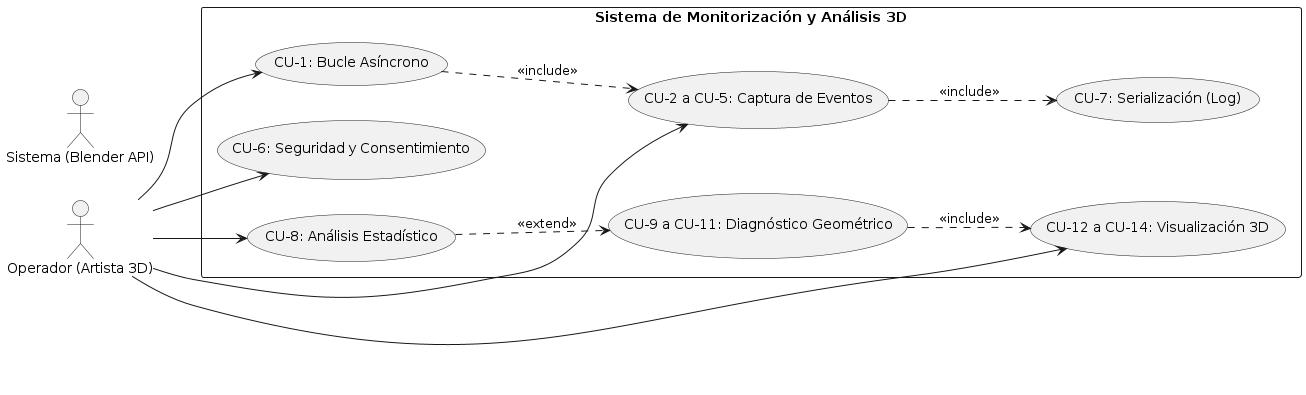
\includegraphics[width=0.95\textwidth]{diagramas/casos_uso_b.png}
    \caption{Diagrama de casos de uso del sistema de monitorización, análisis y visualización.}
    \label{fig:diagrama_cu}
\end{figure}

A continuación se describen los casos de uso principales. Se ha conservado el nivel de detalle necesario para justificar el comportamiento del sistema, pero se evita incluir secuencias excesivamente dependientes de funciones internas concretas. Los nombres de operadores o variables se citan únicamente cuando ayudan a reconocer la correspondencia con la implementación.

% CU-01
\begin{table}[H]
\centering
\scriptsize
\begin{tabularx}{\linewidth}{p{0.23\linewidth}X}
\toprule
\textbf{CU-01} & Inicializar monitorización no intrusiva \\
\midrule
\textbf{Requisitos asociados} & RF-01 a RF-04, RF-17, RF-22, RF-24, RNF-01, RNF-02, RLE-01 \\
\textbf{Descripción} & El sistema inicia un temporizador periódico que evalúa el estado de la escena sin bloquear la interfaz de Blender ni alterar el flujo de modelado. \\
\textbf{Precondición} & El usuario ha aceptado el consentimiento y activa el control de inicio en el panel del Data Logger. \\
\textbf{Secuencia principal} & El sistema cambia el estado de captura a activo, registra el instante inicial, prepara las estructuras de comparación y comienza a muestrear la escena de forma periódica. \\
\textbf{Postcondición} & La sesión queda en estado de escucha activa y preparada para registrar cambios relevantes. \\
\textbf{Excepciones} & El consentimiento no ha sido aceptado, la ejecución automática está deshabilitada o Blender impide registrar el temporizador. \\
\textbf{Prioridad} & Alta \\
\bottomrule
\end{tabularx}
\caption{CU-01: Inicializar monitorización no intrusiva.}
\label{tab:cu1}
\end{table}

% CU-02
\begin{table}[H]
\centering
\scriptsize
\begin{tabularx}{\linewidth}{p{0.23\linewidth}X}
\toprule
\textbf{CU-02} & Auditar cambios topológicos de la malla \\
\midrule
\textbf{Requisitos asociados} & RF-05, RF-06, RF-07, RF-17, RF-18, RNF-03, RNF-04, RNF-06 \\
\textbf{Descripción} & El sistema compara el estado topológico de la malla activa para detectar variaciones en vértices, triángulos, no cuadrángulos y normales potencialmente invertidas. \\
\textbf{Precondición} & Existe un objeto de tipo malla activo y la captura se encuentra iniciada. \\
\textbf{Secuencia principal} & El sistema obtiene la información geométrica disponible, emplea estructuras adecuadas según el modo de trabajo, contrasta los valores con el snapshot anterior y registra solo las diferencias relevantes. \\
\textbf{Postcondición} & Las variaciones topológicas quedan disponibles para su escritura incremental en el CSV. \\
\textbf{Excepciones} & No hay malla activa, se produce un cambio de modo durante la lectura o la geometría no contiene datos válidos. \\
\textbf{Prioridad} & Alta \\
\bottomrule
\end{tabularx}
\caption{CU-02: Auditar cambios topológicos de la malla.}
\label{tab:cu2}
\end{table}

% CU-03
\begin{table}[H]
\centering
\scriptsize
\begin{tabularx}{\linewidth}{p{0.23\linewidth}X}
\toprule
\textbf{CU-03} & Detectar operadores de teclado relevantes \\
\midrule
\textbf{Requisitos asociados} & RF-11, RF-12, RF-13, RF-14, RF-18, RNF-02, RNF-04 \\
\textbf{Descripción} & El sistema identifica operaciones frecuentes de modelado asociadas a combinaciones de teclado, como pegado, duplicación enlazada, duplicación no enlazada y fusión de elementos. \\
\textbf{Precondición} & El Data Logger está activo y los operadores o atajos relevantes se encuentran registrados. \\
\textbf{Secuencia principal} & El usuario ejecuta una acción como \textit{Ctrl+V}, \textit{Shift+D}, \textit{Alt+D} o \textit{Merge}; el sistema marca el evento, actualiza las banderas correspondientes y fuerza el registro de la operación en la siguiente fila válida. \\
\textbf{Postcondición} & La operación queda reflejada en el registro cronológico y puede utilizarse posteriormente en las métricas de actividad. \\
\textbf{Excepciones} & El atajo entra en conflicto con otra herramienta, se modifica el mapa de teclas o la operación no queda expuesta de forma fiable por la API. \\
\textbf{Prioridad} & Media \\
\bottomrule
\end{tabularx}
\caption{CU-03: Detectar operadores de teclado relevantes.}
\label{tab:cu3}
\end{table}

% CU-04
\begin{table}[H]
\centering
\scriptsize
\begin{tabularx}{\linewidth}{p{0.23\linewidth}X}
\toprule
\textbf{CU-04} & Capturar transformaciones espaciales del objeto activo \\
\midrule
\textbf{Requisitos asociados} & RF-02, RF-03, RF-04, RF-17, RF-18, RNF-01, RNF-03 \\
\textbf{Descripción} & El sistema monitoriza los cambios de posición, escala, radio y contexto espacial asociados al objeto activo y a la escena. \\
\textbf{Precondición} & La captura está activa y existe un objeto seleccionado o una escena con objetos de tipo malla. \\
\textbf{Secuencia principal} & El sistema consulta las propiedades espaciales relevantes, las compara con el estado previo mediante tolerancias y registra los deltas cuando existe una modificación significativa. \\
\textbf{Postcondición} & Los cambios espaciales se incorporan al registro de sesión sin almacenar filas redundantes. \\
\textbf{Excepciones} & El objeto activo desaparece, se elimina la malla durante la captura o las transformaciones no pueden leerse temporalmente. \\
\textbf{Prioridad} & Alta \\
\bottomrule
\end{tabularx}
\caption{CU-04: Capturar transformaciones espaciales del objeto activo.}
\label{tab:cu4}
\end{table}

% CU-05
\begin{table}[H]
\centering
\scriptsize
\begin{tabularx}{\linewidth}{p{0.23\linewidth}X}
\toprule
\textbf{CU-05} & Registrar cambios de modo y contexto de trabajo \\
\midrule
\textbf{Requisitos asociados} & RF-06, RF-08, RF-17, RF-18, RNF-04 \\
\textbf{Descripción} & El sistema detecta transiciones entre modos de trabajo, especialmente entre \textit{Object Mode} y \textit{Edit Mode}, para contextualizar las operaciones de modelado. \\
\textbf{Precondición} & La monitorización está activa y Blender informa correctamente del modo de contexto. \\
\textbf{Secuencia principal} & El usuario cambia de modo; el sistema compara el modo actual con el anterior y registra la transición junto con la marca temporal correspondiente. \\
\textbf{Postcondición} & El cambio contextual queda registrado y puede emplearse en métricas relacionadas con estados de trabajo. \\
\textbf{Excepciones} & Pérdida temporal de foco, cambio de área de Blender o consulta de contexto no válida. \\
\textbf{Prioridad} & Media \\
\bottomrule
\end{tabularx}
\caption{CU-05: Registrar cambios de modo y contexto de trabajo.}
\label{tab:cu5}
\end{table}

% CU-06
\begin{table}[H]
\centering
\scriptsize
\begin{tabularx}{\linewidth}{p{0.23\linewidth}X}
\toprule
\textbf{CU-06} & Gestionar consentimiento y seudonimización \\
\midrule
\textbf{Requisitos asociados} & RF-22, RF-23, RLE-01, RLE-02, RLE-03, RLE-04 \\
\textbf{Descripción} & El sistema solicita aceptación explícita antes de iniciar la captura y evita almacenar identificadores personales directos. \\
\textbf{Precondición} & El add-on se encuentra instalado o cargado en Blender. \\
\textbf{Secuencia principal} & El sistema comprueba si existe aceptación previa; si no existe, muestra el aviso correspondiente, bloquea la captura y solo permite continuar tras la aceptación informada. \\
\textbf{Postcondición} & La captura queda habilitada o bloqueada según el estado del consentimiento. \\
\textbf{Excepciones} & No se puede guardar la preferencia local o el usuario rechaza el consentimiento. \\
\textbf{Prioridad} & Alta \\
\bottomrule
\end{tabularx}
\caption{CU-06: Gestionar consentimiento y seudonimización.}
\label{tab:cu6}
\end{table}

% CU-07
\begin{table}[H]
\centering
\scriptsize
\begin{tabularx}{\linewidth}{p{0.23\linewidth}X}
\toprule
\textbf{CU-07} & Persistir y exportar el registro CSV \\
\midrule
\textbf{Requisitos asociados} & RF-18, RF-19, RF-20, RF-21, RLE-05, RIU-03, RNF-09 \\
\textbf{Descripción} & El sistema conserva los datos registrados durante la sesión y permite exportarlos a un fichero CSV externo. \\
\textbf{Precondición} & Existen filas registradas o un bloque interno recuperable dentro del archivo \texttt{.blend}. \\
\textbf{Secuencia principal} & El sistema mantiene el registro incremental, puede incrustar una copia interna en el proyecto y exporta el CSV cuando el usuario lo solicita mediante la interfaz. \\
\textbf{Postcondición} & El registro queda disponible como archivo externo para su análisis posterior. \\
\textbf{Excepciones} & Fallo de escritura, permisos insuficientes, ruta no válida o ausencia de registros exportables. \\
\textbf{Prioridad} & Alta \\
\bottomrule
\end{tabularx}
\caption{CU-07: Persistir y exportar el registro CSV.}
\label{tab:cu7}
\end{table}

% CU-08
\begin{table}[H]
\centering
\scriptsize
\begin{tabularx}{\linewidth}{p{0.23\linewidth}X}
\toprule
\textbf{CU-08} & Cargar y validar colecciones de CSV \\
\midrule
\textbf{Requisitos asociados} & RF-26, RF-27, RF-28, RNF-05, RNF-11 \\
\textbf{Descripción} & El add-on de análisis localiza uno o varios CSV, comprueba su estructura y prepara los datos para el cálculo de métricas. \\
\textbf{Precondición} & El usuario selecciona un archivo o carpeta con registros generados por el Data Logger. \\
\textbf{Secuencia principal} & El sistema detecta los CSV, lee sus cabeceras y valores, descarta o informa de datos no válidos y carga en memoria las series numéricas utilizables. \\
\textbf{Postcondición} & Los datos quedan preparados para el análisis estadístico y la visualización. \\
\textbf{Excepciones} & CSV vacío, columnas ausentes, codificación incompatible o valores no finitos. \\
\textbf{Prioridad} & Alta \\
\bottomrule
\end{tabularx}
\caption{CU-08: Cargar y validar colecciones de CSV.}
\label{tab:cu8}
\end{table}

% CU-09
\begin{table}[H]
\centering
\scriptsize
\begin{tabularx}{\linewidth}{p{0.23\linewidth}X}
\toprule
\textbf{CU-09} & Calcular métricas estadísticas A1--A17 \\
\midrule
\textbf{Requisitos asociados} & RF-29 a RF-34, RIU-06, RIU-07, RIU-08, RIU-10, RIU-12 \\
\textbf{Descripción} & El sistema calcula las métricas estadísticas de la sesión o conjunto de sesiones, aplicando agrupaciones y cuartiles selectivos cuando corresponda. \\
\textbf{Precondición} & Existen datos CSV validados. \\
\textbf{Secuencia principal} & El usuario solicita el cálculo; el sistema obtiene la duración en horas, actividad general, pausas, picos, velocidades, tamaños locales, transiciones y métricas de eventos, agrupando A2--A3 y A6--A9 cuando procede y manteniendo separadas A12, A13 y A16. \\
\textbf{Postcondición} & Las métricas A1--A17 quedan disponibles para su presentación en paneles. \\
\textbf{Excepciones} & Series temporales incompletas, duración nula o ausencia de columnas necesarias. \\
\textbf{Prioridad} & Alta \\
\bottomrule
\end{tabularx}
\caption{CU-09: Calcular métricas estadísticas A1--A17.}
\label{tab:cu9}
\end{table}

% CU-10
\begin{table}[H]
\centering
\scriptsize
\begin{tabularx}{\linewidth}{p{0.23\linewidth}X}
\toprule
\textbf{CU-10} & Calcular similitud geométrica y distancia de Hausdorff \\
\midrule
\textbf{Requisitos asociados} & RF-43, RF-44, RF-45, RF-46, RNF-06, RNF-12 \\
\textbf{Descripción} & El sistema compara un objeto con una referencia para estimar similitud geométrica, similitud topológica y distancia de Hausdorff o una aproximación equivalente cuando resulte aplicable. \\
\textbf{Precondición} & Existe un objeto seleccionado y, si la métrica lo requiere, un objeto de referencia válido. \\
\textbf{Secuencia principal} & El sistema obtiene coordenadas transformadas al espacio global, compara vértices y estructura topológica, penaliza diferencias relevantes y calcula el indicador de similitud o distancia. \\
\textbf{Postcondición} & Los resultados de comparación quedan disponibles en el panel de análisis. \\
\textbf{Excepciones} & Ausencia de referencia, geometría sin vértices válidos, diferencias extremas de escala o mallas no comparables. \\
\textbf{Prioridad} & Alta \\
\bottomrule
\end{tabularx}
\caption{CU-10: Calcular similitud geométrica y distancia de Hausdorff.}
\label{tab:cu10}
\end{table}

% CU-11
\begin{table}[H]
\centering
\scriptsize
\begin{tabularx}{\linewidth}{p{0.23\linewidth}X}
\toprule
\textbf{CU-11} & Analizar mapas UV \\
\midrule
\textbf{Requisitos asociados} & RF-36, RF-37, RF-38, RF-39, RNF-06, RNF-12 \\
\textbf{Descripción} & El sistema evalúa la capa UV activa para calcular área UV, número de islas, deformación y densidad de texeles. \\
\textbf{Precondición} & El objeto seleccionado posee una malla con coordenadas UV válidas. \\
\textbf{Secuencia principal} & El sistema consulta la capa UV activa, recorre la conectividad de las coordenadas, estima áreas o relaciones geométricas y presenta las métricas resultantes. \\
\textbf{Postcondición} & Las métricas UV se incorporan al bloque correspondiente de resultados. \\
\textbf{Excepciones} & Objeto sin UV, capa UV vacía, caras degeneradas o coordenadas inconsistentes. \\
\textbf{Prioridad} & Media \\
\bottomrule
\end{tabularx}
\caption{CU-11: Analizar mapas UV.}
\label{tab:cu11}
\end{table}

% CU-12
\begin{table}[H]
\centering
\scriptsize
\begin{tabularx}{\linewidth}{p{0.23\linewidth}X}
\toprule
\textbf{CU-12} & Diagnosticar normales, ángulos y estructura de malla \\
\midrule
\textbf{Requisitos asociados} & RF-35, RF-40, RF-41, RF-42, RF-43, RNF-06, RNF-12 \\
\textbf{Descripción} & El sistema calcula métricas de calidad geométrica relacionadas con normales, ángulos entre caras, polígonos no cuadrangulares y vértices duplicados. \\
\textbf{Precondición} & Existe una malla seleccionada y evaluable. \\
\textbf{Secuencia principal} & El sistema inspecciona la geometría, calcula porcentajes o recuentos relevantes y genera indicadores de diagnóstico para apoyar la interpretación de la calidad del modelo. \\
\textbf{Postcondición} & Los resultados geométricos quedan visibles en el panel de análisis. \\
\textbf{Excepciones} & Malla vacía, caras degeneradas, normales nulas o datos no aplicables al tipo de objeto. \\
\textbf{Prioridad} & Media \\
\bottomrule
\end{tabularx}
\caption{CU-12: Diagnosticar normales, ángulos y estructura de malla.}
\label{tab:cu12}
\end{table}

% CU-13
\begin{table}[H]
\centering
\scriptsize
\begin{tabularx}{\linewidth}{p{0.23\linewidth}X}
\toprule
\textbf{CU-13} & Generar gráficos estadísticos 2D \\
\midrule
\textbf{Requisitos asociados} & RF-47, RIU-05, RIU-07, RIU-08, RIU-10, RNF-07 \\
\textbf{Descripción} & El sistema genera representaciones gráficas bidimensionales a partir de las series de datos procesadas, integrándolas en Blender cuando sea necesario. \\
\textbf{Precondición} & Existen datos numéricos válidos y se ha seleccionado un tipo de gráfico compatible. \\
\textbf{Secuencia principal} & El usuario solicita una visualización; el sistema prepara los vectores de datos, genera el gráfico mediante una librería de representación y lo muestra como resultado asociado a la sesión. \\
\textbf{Postcondición} & El gráfico queda disponible para la interpretación visual de las métricas. \\
\textbf{Excepciones} & Datos insuficientes, tipo de gráfico incompatible o error de renderizado. \\
\textbf{Prioridad} & Media \\
\bottomrule
\end{tabularx}
\caption{CU-13: Generar gráficos estadísticos 2D.}
\label{tab:cu13}
\end{table}

% CU-14
\begin{table}[H]
\centering
\scriptsize
\begin{tabularx}{\linewidth}{p{0.23\linewidth}X}
\toprule
\textbf{CU-14} & Crear visualizaciones procedurales 3D en Blender \\
\midrule
\textbf{Requisitos asociados} & RF-48, RF-49, RF-50, RNF-07, RNF-08, RIU-05 \\
\textbf{Descripción} & El sistema traduce resultados analíticos en elementos visuales tridimensionales dentro de la escena de Blender, como nubes de puntos, superficies o mapas de radar. \\
\textbf{Precondición} & Existen métricas calculadas y una visualización tridimensional aplicable. \\
\textbf{Secuencia principal} & El sistema limpia visualizaciones anteriores si procede, calcula posiciones o relaciones espaciales, genera la geometría procedural y asigna materiales o etiquetas necesarias para su lectura. \\
\textbf{Postcondición} & La visualización queda integrada en la escena y puede inspeccionarse desde Blender. \\
\textbf{Excepciones} & Datos nulos, escala no representable, fallo al crear geometría o ausencia de contexto de escena válido. \\
\textbf{Prioridad} & Media \\
\bottomrule
\end{tabularx}
\caption{CU-14: Crear visualizaciones procedurales 3D en Blender.}
\label{tab:cu14}
\end{table}

\section{Trazabilidad entre casos de uso y requisitos}

\begin{table}[H]
\centering
\scriptsize
\begin{tabularx}{\textwidth}{p{2.5cm}X}
\toprule
\textbf{Caso de uso} & \textbf{Requisitos asociados} \\
\midrule
CU-01 & RF-01 a RF-04, RF-17, RF-22, RF-24, RNF-01, RNF-02, RLE-01 \\
CU-02 & RF-05, RF-06, RF-07, RF-17, RF-18, RNF-03, RNF-04, RNF-06 \\
CU-03 & RF-11 a RF-14, RF-18, RNF-02, RNF-04 \\
CU-04 & RF-02, RF-03, RF-04, RF-17, RF-18, RNF-01, RNF-03 \\
CU-05 & RF-06, RF-08, RF-17, RF-18, RNF-04 \\
CU-06 & RF-22, RF-23, RLE-01 a RLE-04 \\
CU-07 & RF-18 a RF-21, RLE-05, RIU-03, RNF-09 \\
CU-08 & RF-26, RF-27, RF-28, RNF-05, RNF-11 \\
CU-09 & RF-29 a RF-34, RIU-06 a RIU-08, RIU-10, RIU-12 \\
CU-10 & RF-43 a RF-46, RNF-06, RNF-12 \\
CU-11 & RF-36 a RF-39, RNF-06, RNF-12 \\
CU-12 & RF-35, RF-40 a RF-43, RNF-06, RNF-12 \\
CU-13 & RF-47, RIU-05, RIU-07, RIU-08, RIU-10, RNF-07 \\
CU-14 & RF-48, RF-49, RF-50, RNF-07, RNF-08, RIU-05 \\
\bottomrule
\end{tabularx}
\caption{Trazabilidad entre casos de uso y requisitos.}
\label{tab:trazabilidad_cu_rf}
\end{table}

